\documentclass{beamer}

\usepackage{Haust2016glærur}

\title{Stærðfræðimynstur í tölvunarfræði}
\subtitle{Vika 4, fyrri fyrirlestur}

\begin{document}

\begin{frame}
\titlepage
\end{frame}


\section{Inngangur}

\begin{frame}{Í síðasta tíma}
\begin{itemize}
 \item Reikniflækja
 \item Tímaflækjur nokkurra reiknirita
 \item Mengin $P$ og $NP$
\end{itemize}
\end{frame}

\section{Talnafræði}

\begin{frame}{Talnafræði}
\begin{itemize}
 \item Stærðfræði heiltalna kallast talnafræði
 \item Löng og mikil saga
 \begin{itemize}
  \item Fræg forn-grísk nöfn sem koma við sögu: Evklíð, Eratosþenes
 \end{itemize}
 \item Stærðfræði prímtalna fellur undir talnafræði
\end{itemize}
\end{frame}

\section{Deiling og afgangur}

\begin{frame}{Deilanleiki}
Ýmis hugtök í talnafræði krefjast skilnings á deilanleika (e. \emph{divisibility})

\begin{tcolorbox}[title=Deilanleiki]
Séu $a$ og $b$ heiltölur, $a \neq 0$, segjum við að $a$ deili (e. \emph{divides}) $b$ ef til er heiltala $c$ svo að $b = ac$, þ.e.a.s. ef $\frac{b}{a}$ er heiltala.

Þegar $a$ deilir $b$ segjum við að $a$ sé deilir (e. \emph{divisor} eða \emph{factor}) $b$ og að $b$ sé margfeldi (e. \emph{multiple}) af $a$.

Við skrifum $a | b$ þegar $a$ deilir $b$, annars $a \nmid b$.
\end{tcolorbox}
\end{frame}

\begin{frame}{Deilanleiki - dæmi}
Er $3|7$? \pause

Nei, $7/3$ er ekki heiltala. \pause

\vspace{0.5cm}
Er $3|12$? \pause

Já, $12/3$ er heiltalan $4$.
\end{frame}

\begin{frame}{Eiginleikar deilanleika}
Heiltöludeiling hefur nokkra áhugaverða eiginleika
\begin{tcolorbox}[title=Eiginleikar deilanleika]
Séu $a$, $b$ og $c$ heiltölur, $a \neq 0$, þá gildir:
\begin{enumerate}
 \item Sé $a|b$ og $a|c$, þá $a|(b+c)$
 \item Sé $a|b$, þá $a|b\cdot c$
 \item Sé $a|b$ og $b|c$, þá $a|c$
\end{enumerate}
\end{tcolorbox}
\end{frame}

\begin{frame}{Deilingarreikniritið}
Deilingarreikniritið er ekki reiknirit, heldur setning.

\begin{tcolorbox}[title=Deilingarreikniritið]
Látum $a$ og $d$ vera heiltölur, $d > 0$. 
Þá eru til heiltölur $q$ og $r$, $0 \leq r < d$ svo að $a = dq +r$.
\end{tcolorbox}

Hér er $d$ deilir, $a$ deilistofn (e. \emph{dividend}), $q$ kvóti (e. \emph{quotient}) og $r$ afgangur (e. \emph{remainder}).
\end{frame}


\begin{frame}{Kvóti og afgangur}
Um deilinn $d$, deilistofninn $a$, kvótann $q$ og afganginn $r$ má rita:
\[
 q = a \text{ div } d
\]
og
\[
 r = a \text{ mod } d
\]
\end{frame}

\begin{frame}{Dæmi um deilingu}
Hverjir eru kvótinn og afgangurinn þegar deilistofninn er $101$ og deilirinn $11$ (þ.e.a.s. reiknum 101/11)? \pause

Höfum
\[
 101 = 11 \cdot 9 + 2
\]

Svo kvótinn er $101 \text{ div } 11 = 9$ og afgangurinn $101 \Mod 11 = 2$.

\end{frame}

\begin{frame}{Dæmi um deilingu}
Hverjir eru kvótinn og afgangurinn þegar deilistofninn er $-11$ og deilirinn $3$ (þ.e.a.s. reiknum 11/3)? \pause

Höfum
\[
 -11 = 3 \cdot (-4) + 1
\]

Svo kvótinn er $-11 \text{ div } 3 = -4$ og afgangurinn $-11 \Mod 3 = 1$.

\vspace{0.5cm}
Athugum að þó að $-11 = 3(-3) - 2$ sé satt, þá uppfyllir jafnan ekki $0 \leq r < 3$.
\end{frame}

\begin{frame}{Varúð - forritunarmál}
\begin{itemize}
 \item Forritunarmál meðhöndla deilingarafgang á ýmsa vegu
 \begin{itemize}
  \item Stundum virki (\%)
  \item Stundum föll (\texttt{mod} eða \texttt{rem})
  \item Stundum meira en eitt fall\ldots
 \end{itemize}
 \item Neikvæðar tölur sérstaklega varhugaverðar
 \begin{itemize}
  \item Stundum er deilingarafganginum leyft að vera neikvæður
  \item Stundum er $a \Mod m$ skilgreint jafnvel þó að $m$ sé neikvætt eða 0
 \end{itemize}
\end{itemize}
\end{frame}

\section{Framsetning heiltalna}

\begin{frame}{Framsetning heiltalna}
\begin{itemize}
 \item Fólk í flestum menningarheimum notar tugakerfið til að setja fram tölur
 \begin{itemize}
  \item Líklega vegna þess að við höfum 10 fingur
  \item Hafa eiginleika sem byggjast á tölunni 10: $965 = 9\cdot10^2+6\cdot10^1+5\cdot10^0$
 \end{itemize}
 \item Tölvuútreikningar byggjast oftast á grunntölunni 2 (tvíundarkerfi)
 \begin{itemize}
  \item Einnig til áttundakerfi (e. \emph{octal}) með grunntöluna 8 og sextándakerfi (e. \emph{hexadecimal}) með grunntöluna 16
  \item Áttunda- og sextándakerfistölur eru oftast notaðar til að setja tvíundarkerfistölur fram fyrir fólk
 \end{itemize}
\end{itemize}
\end{frame}

\begin{frame}{Framsetning heiltalna}
Um framsetningu heiltalna gildir:

\begin{tcolorbox}[title=Framsetning heiltalna]
Látum $b$ vera heiltölu, $b > 1$. Þá getum við sett fram jákvæðu heiltöluna $n$ á sniðinu
\[
 n = a_kb^k + a_{k-1}b^{k-1} + \ldots + a_1b + a_0
\]
þar sem $k$ er ekki-neikvæð heiltala, $a_0, a_1, \ldots, a_k$ eru ekki-neikvæðar heiltölur minni en $b$ og $a_k \neq 0$.
\end{tcolorbox}
Talað er um framsetningu með grunntölunni $b$.
\end{frame}

\begin{frame}{Reiknirit til grunntöluskipta}
Gráðugt reiknirit má nota til að skipta um grunntölu:
\begin{center}
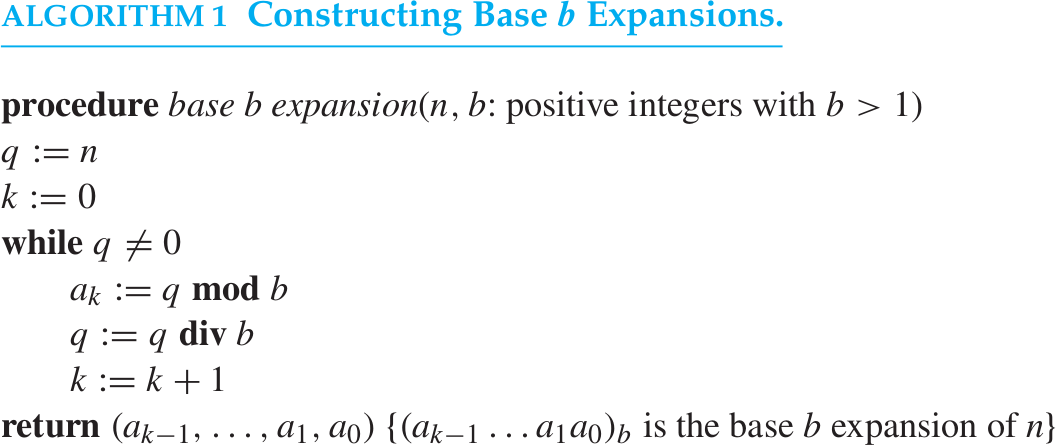
\includegraphics[width=\textwidth]{base-conversion-algorithm}
\end{center}
\end{frame}

\begin{frame}{Grunntöluskipti - dæmi}
\vspace{0.5cm}
Setjum tugakerfistöluna $(241)_{10}$ fram sem tvíundakerfistölu.
\begin{align*}
241 &= 2 \cdot 120 + 1\\
120 &= 2 \cdot 60 + 0\\
60 &= 2 \cdot 30 + 0\\
30 &= 2 \cdot 15 + 0\\
15 &= 2 \cdot 7 + 1\\
3 &= 2 \cdot 1 + 1\\
1&= 2 \cdot 0 + 1\\
\end{align*}

\vspace{-0.8cm}
Fáum afgangana $1, 0, 0, 0, 1, 1, 1, 1$ svo
\[
 (241)_{10} = (11110001)_2
\]
\end{frame}

\begin{frame}{Samlagning tvíundartalna}
Reikniaðgerðir með heiltölur fara fram með svipuðum hætti óháð framsetningu þeirra.
\begin{center}
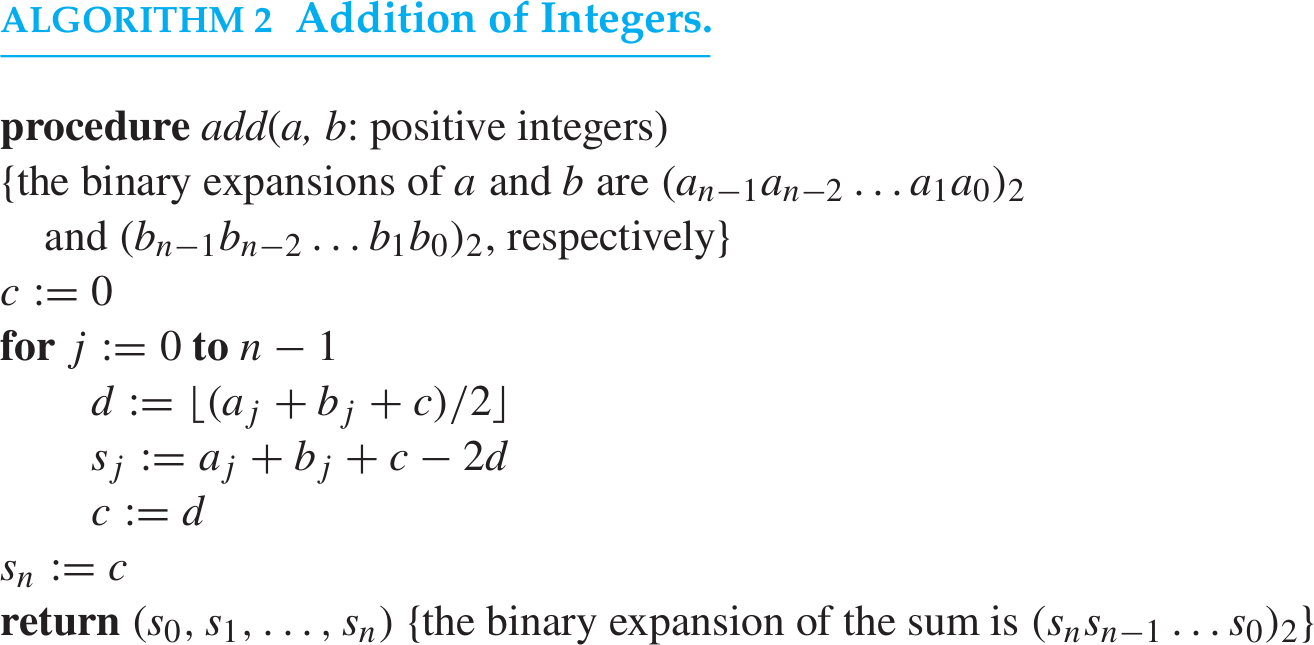
\includegraphics[width=0.9\textwidth]{binary-addition}
\end{center}
\end{frame}

\begin{frame}{Veldishafning og afgangar}
\begin{itemize}
 \item Stundum þarf að reikna út $b^n \Mod m$, þar sem $b$, $n$ og $m$ eru stórar heiltölur
 \item Ekki er skilvirkt að reikna fyrst út $b^n$ og svo afganginn þegar deilt er með $m$, því $b^n$ verður risastór tala
 \item Til að einfalda útreikninga notum við tvíundarframsetningu á $n$, $n = (a_{k-1}\ldots a_1 a_0)_2$ til að setja fram $b^n$
\end{itemize}
\[
 b_n = b^{a_{k-1}\cdot 2^{k-1} + \ldots + a_1\cdot 2^1 + a_0 \cdot 2^0} = b^{a_{k-1}\cdot2^{k-1}\cdot \ldots \cdot b^{a_1\cdot 2} \cdot b^{a_0}}
\]
Margföldum saman þá liði þar sem tvíundarframsetningin á $n$ er með 1.
\end{frame}

\begin{frame}{Dæmi: Framsetning á $3^{11}$}
Athugum að $(11)_{10} = (1011)_2$ og sjáum:
\begin{align*}
3^{11} &= 3^8\cdot 3^2 \cdot 3^1\\
&=6561 \cdot 9 \cdot 3\\
&=177147
\end{align*}

\end{frame}

\begin{frame}{Modular exponentiation}
Notum þessa innsýn til að setja fram reiknirit til að reikna $b^n \Mod m$:
\begin{center}
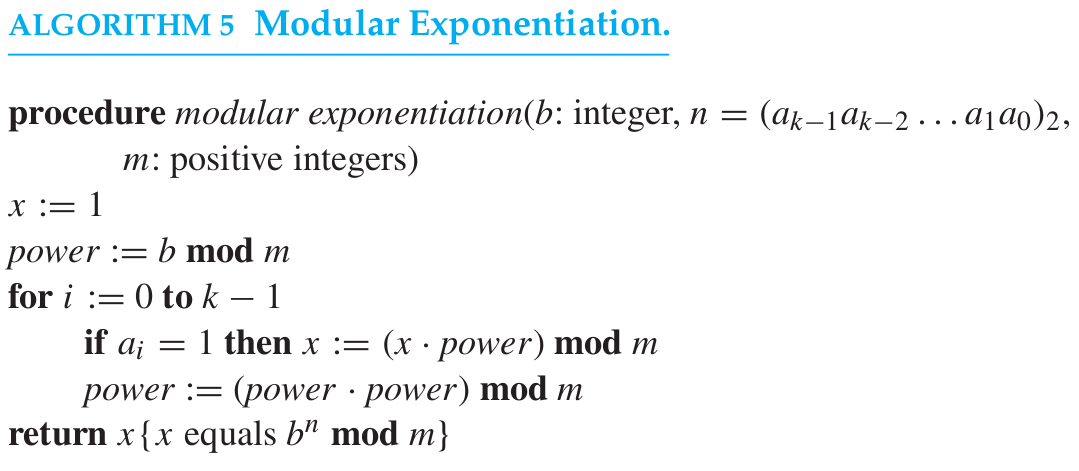
\includegraphics[width=0.9\textwidth]{modular-exponentiation}
\end{center}
\end{frame}

\section{Prímtölur}

\begin{frame}{Prímtölur}
\begin{tcolorbox}[title=Prímtölur]
Heiltala $p$ stærri en 1 er prímtala (e. \emph{prime}) ef einu deilar $p$ eru 1 og $p$ sjálft. Heiltala stærri en 1 sem ekki er prímtala er samsett tala (e. \emph{composite}).
\end{tcolorbox}
\end{frame}


\begin{frame}{Grundvallarsetning}
``The fundamental theorem of arithmetic'' er eftirfarandi:

\begin{tcolorbox}[title=Fundamental theorem of arithmetic]
Hver heiltala stærri en 1 er prímtala eða margfeldi tveggja eða fleiri prímtalna sem skrifa má í stígandi röð.
\end{tcolorbox}

Það að finna prímtölurnar sem mynda samsetta tölu þegar þær eru margfaldaðar saman kallast að finna prímtöluþætti samsettu tölunnar.
\end{frame}

\begin{frame}{Að finna prímtöluþætti}
Erfitt verk er að finna prímtöluþætti. Einfaldasta leiðin er að prófa margar deilingar. Þá er eftirfarandi staðreynd gagnleg:
\begin{tcolorbox}
Sé $n$ samsett heiltala, þá á $n$ prímtöluþátt minni en eða jafnan $\sqrt{n}$
\end{tcolorbox}
\end{frame}

\begin{frame}{Prímtöluþáttun: Dæmi}
Sýnum að 101 sé prímtala.

Einu prímtölurnar sem eru minni en $\sqrt{101}$ eru $2, 3, 5$ og $7$. Þar sem engin þessara talna myndar heiltölukvóta þegar $101$ er deilt með þeim er $101$ prímtala.
\end{frame}

\begin{frame}{Prímtöluþáttun: Dæmi}
Finnum prímtöluþáttun 7007. Prófum að deila með prímtölum í vaxandi röð.

2, 3 og 5 ganga ekki upp í 7007, en 7 gerir það og gefur kvótann 1001. Byrjum aftur á að deila með 7 og fáum 1001/7 = 143. 7 gengur ekki upp í 143, en 143/11 = 13. 13 er prímtala, svo við erum búin. Prímtöluþáttunin er $7 \cdot 7 \cdot 11 \cdot 13$.
\end{frame}

\begin{frame}{Prímtöluþáttun - hversu erfið?}
Deiling verður mjög þung aðgerð þegar fjöldi bita er stór, endurteknar deilingar þeim mun verri. M.t.t. fjölda bita vex keyrslutíminn veldisvexti. Ekkert reiknirit er til sem finnur prímtöluþáttun á margliðutíma.

Skilvirkasta þáttunarreiknritið sem þekkt er, GNFS, þáttar $b$ bita heiltölu á 
\[
 O \left(exp\left(\sqrt[3]{\frac{64}{9}b(\log b)^2}\right)\right)
\]
sem er samt ekki margliðutími. Þetta atriði er mikilvægt í dulkóðun.
\end{frame}

\begin{frame}{Prímtölutékk - hversu erfitt?}
\begin{itemize}
 \item Hægt er að nota endurtekna deilingu til að athuga hvort að tala sé prímtala
 \begin{itemize}
  \item Veldisvísistími
 \end{itemize}
 \item Ýmis góð reiknirit til
 \item Hægt er að komast að því hvort að tala sé prímtala eða ekki á margliðutíma
 \begin{itemize}
  \item Agrawal-Kayal-Saxena (AKS) primality test, 2002
  \item Merkileg niðurstaða!
 \end{itemize}
\end{itemize}
\end{frame}

\section{Stærsti samdeilir og minnsta samfeldi}

\begin{frame}{Stærsti samdeilir}
\begin{tcolorbox}[title=Stærsti samdeilir]
Látum $a$ og $b$ vera heiltölur, ekki báðar núll. Stærsta heiltala $d$ svo að $d|a$ og $d|b$ er kölluð stærsti samdeilir (e. \emph{greatest common divisor}) $a$ og $b$ og táknuð með $gcd(a, b)$.
\end{tcolorbox}
Dæmi: $gcd(24, 36) = 12$

Tvær tölur með stærsta samdeilinn 1 eru ósamþátta (e. \emph{relatively prime}). Hægt er að reikna út stærsta samdeili með reikniriti Evklíðs (sjá bók).
\end{frame}

\begin{frame}{Minnsta samfeldi}
\begin{tcolorbox}[title=Minnsta samfeldi]
Minnsta samfeldi (e. \emph{least common multiple}) jákvæðra heiltalna $a$ og $b$ er minnsta jákvæða heiltala sem er deilanleg með bæði $a$ og $b$. Hún er táknuð $lcm(a, b)$.
\end{tcolorbox}
Dæmi: $lcm(4, 6) = 12$.
\end{frame}

\begin{frame}{Tengsl GCD og LCM}
\begin{tcolorbox}[title=GCD og LCM]
Látum $a$ og $b$ vera jákvæðar heiltölur. Þá er $a\cdot b = gcd(a, b) \cdot lcm(a, b)$.
\end{tcolorbox}
\end{frame}



\begin{frame}{Næst}
Dulkóðun (4.6)

Seinni helmingur tímans er stoðtími.
\end{frame}


\end{document}
